\begin{center}
	\Huge
	Lineær regression og residualer
\end{center}
\section*{Kvalitet af lineær model}
\stepcounter{section}

Vi har tidligere set på residualplots for at afgøre kvaliteten af en lineær model på et datasæt. Vi har nu et bedre værktøj til at afgøre, hvor god en regressionsmodel passer på et datasæt - fraktilplottet. 

\begin{exa}
	155 personer har målt deres makspuls. Sammenhængen mellem deres alder og makspuls fremgår af \href{}{\color{blue!60} dette datasæt}. Vi laver lineær regression i Maple som
	vi plejer:
	\begin{align*}
		&\texttt{with(Gym):}\\
		&\texttt{alder := [...]}\\
		&\texttt{puls := [...]}\\
		&\texttt{LinReg(alder,puls)}
	\end{align*}
	Resultatet af dette kan ses på Fig. \ref{fig:linreg}.
	\begin{figure}[H]
		\centering
		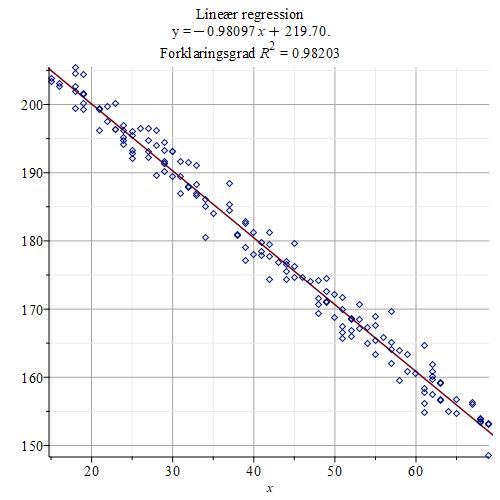
\includegraphics[width=0.7\textwidth]{Billeder/linregpuls.jpg}
		\caption{Lineær regression på pulsdata i Maple}
		\label{fig:linreg}
	\end{figure}
	Af Fig. \ref{fig:linreg} ser regressionen ud til at passe godt til datasættet, men vi fortsætter vores regressionsanalyse. Vi laver først et residualplot som vi plejer. 
	Dette gøres i Maple ved at skrive
	\begin{align*}
		&\texttt{with(Gym):}\\
		&\texttt{alder := [...]}\\
		&\texttt{puls := [...]}\\
		&\texttt{plotResidualer(alder,puls,LinReg)}
	\end{align*}
	Resultatet af dette kan ses på Fig. \ref{fig:linres}
	\begin{figure}[H]
		\centering
		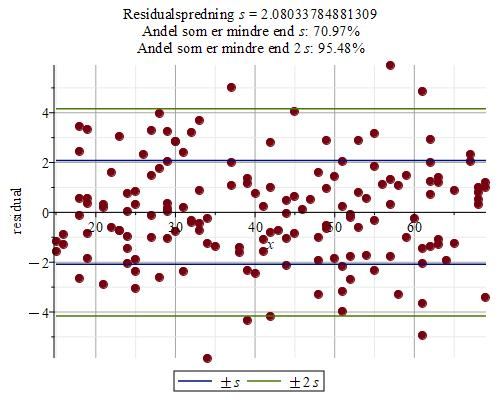
\includegraphics[width=0.7\textwidth]{Billeder/linrespuls.jpg}
		\caption{Residualplot for lineær regression på pulsdata i Maple}
		\label{fig:linres}
	\end{figure}
	Igen ser resultatet fint ud og residualerne ser ud til at være normalfordelte. Vi afslutter med at lave et fraktilplot af residualerne. Dette gøres i Maple som
	\begin{align*}
		&\texttt{with(Gym):}\\
		&\texttt{alder := [...]}\\
		&\texttt{puls := [...]}\\
		&\texttt{residualQQplot(alder,puls,LinReg)}
	\end{align*}
	Resultatet af dette kan ses på Fig. \ref{fig:qqplot}
	\begin{figure}[H]
		\centering
		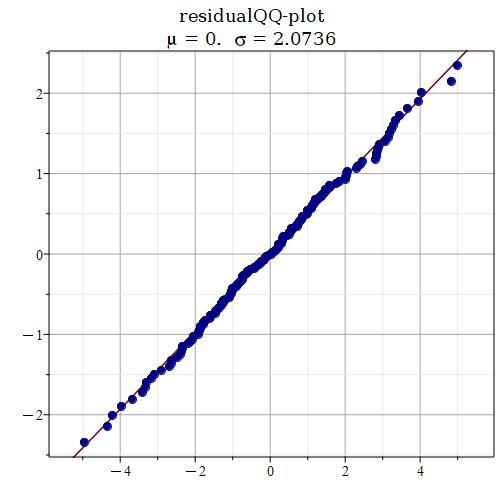
\includegraphics[width=0.7\textwidth]{Billeder/qqplotpuls.jpg}
		\caption{Fraktilplot for residualerne af pulsdata i Maple}
		\label{fig:qqplot}
	\end{figure}
	Residualerne ser ud til at følge den rette linje pænt. Derfor antager vi, at residualerne er normalfordelte og dermed at en lineær model beskriver sammenhængen mellem alder
	og makspuls godt - i hvert fald i vores datas tilfælde. 
	Til slut vil vi gerne bestemme et $95\%$-konfidensinterval for parametrene $a$ og $b$ i vores lineære model 
	\begin{align*}
		y = ax + b.
	\end{align*}		
	Dette gøres i Maple ved at skrive 
	\begin{align*}
		&\texttt{with(Gym):}\\
		&\texttt{alder := [...]}\\
		&\texttt{puls := [...]}\\
		&\texttt{testLin(alder,puls)}
	\end{align*}
	Dette giver os et $95\%$-konfidensinterval for $a$ på
	\begin{align*}
		[-1.00216,-0.95978]
	\end{align*}
	og for $b$
	\begin{align*}
		[218.75654,220.64216].
	\end{align*}
	
\end{exa}

\section*{Opgave 1}

Prisen på en volatil aktie i en tidsperiode på 401 sekunder kan findes i \href{https://github.com/ChristianJLex/TeachingNotes/raw/master/2022-2023/Data%20og%20lign/Aktiepris.xlsx}{\color{blue!60} dette datasæt}.
\begin{enumerate}[label=\roman*)]
	\item Lav lineær regression på datasættet.
	\item Lav et residualplot og overvej, om residualerne ser ud til at være normalfordelte.
	\item Lav et fraktilplot og overvej, om residualerne ser ud til at være normalfordelte. 
	\item Brug modellen til at afgøre, hvornår prisen er 680kr. Bestem sandsynligheden for, at prisen til dette tidspunkt er under 678 kr. 
	\item Bestem et $95\%$-konfidensinterval for $a$ og $b$ i den lineære model. 
\end{enumerate}

\section*{Opgave 2}

250 frø er sået på forskellige tidspunkter og højden på planten er målt efter et antal dage. Sammenhængen mellem alderen og højden kan ses i \href{https://github.com/ChristianJLex/TeachingNotes/raw/master/2022-2023/Data%20og%20lign/Plantevaekst.xlsx}{\color{blue!60} dette datasæt.}

\begin{enumerate}[label=\roman*)]
	\item Lav lineær regression på datasættet.
	\item Lav et residualplot og overvej, om residualerne ser ud til at være normalfordelte.
	\item Lav et fraktilplot og overvej, om residualerne ser ud til at være normalfordelte. 
	\item Hvad er sandsynligheden for, at planten er under 12cm efter 100 dage?
	\item Brug modellen til at afgøre, hvornår planterne er 50cm høje.
	\item Bestem et $95\%$-konfidensinterval for $a$ og $b$ i den lineære model. 
\end{enumerate}

\section*{Opgave 3}
Et studie på 413 personer skal afklare, om et bestemt kosttilskud kan øge den muskelstyrkende effekt af vægttræning. Effekten af træningen måles ved at tage et vægtet gennemsnit
af ydelsen på en række forskellige øvelser. I 
\href{https://github.com/ChristianJLex/TeachingNotes/raw/master/2022-2023/Data%20og%20lign/kosttilskud.xlsx}{\color{blue!60}dette datasæt}
 fremgår ydelsesforskellen sammenlignet med gennemsnittet af en kontrolgruppe, der har udført samme træningsprogram men uden kosttilskud. 

\begin{enumerate}[label=\roman*)]
	\item Lav en lineær regression på datasættet, og afgør, om residualerne er normalfordelte. 
	\item Bestem et $95\%$-konfidensinterval for hældningen $a$ og afgør, om vi kan konkludere, at kosttilskudet har en virkning. 
\end{enumerate}
